\section{Attack}\label{sec:attack}

\begin{figure}
    \centering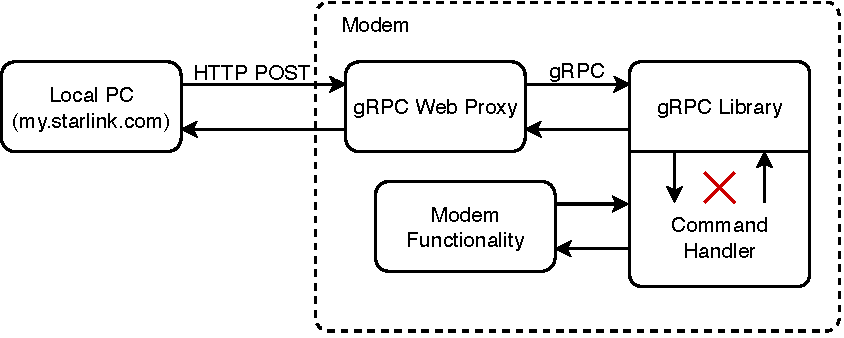
\includegraphics[width=\columnwidth]{img/modem.pdf}
    \caption{Overview of the Starlink modem functionality. gRPC calls are encapsulated within HTTP POST requests by the web interface, which are decoded and processed. Malformed gRPC requests cause the command handler to crash, resulting in the modem no longer being able to respond to commands.}
    \label{fig:modem}
\end{figure}

In this section we explore the underlying architecture of the Starlink modem, and how this opens the system up to denial of service attacks.
We also describe an attack on the command handler resulting in persistent denial of service.

The user terminal is typically administered via the ``\url{http://my.starlink.com}'' web interface.
This interface sends commands to the modem over the local network, using gRPC (Google Remote Procedure Calls) encapsulated within HTTP ``POST'' requests.
As shown in Figure~\ref{fig:modem}, these requests are decoded by a gRPC web proxy, and forwarded to a command handler.

Although typically sent using the web interface, these gRPC commands can also be made on their own from any device or application on the local network.
These commands can be sent directly through tools such as the \textit{grpcurl} command-line interface~\cite{gRPCurl}.
This can also be used to query the modem for available functions.
Alternatively, with prior knowledge of the format and commands, HTTP-encapsulated gRPC requests can be sent directly using tools like \textit{cURL}~\cite{cURL}.
It is not easy to construct these manually, but a network monitor such as \textit{Wireshark} can be used to inspect the bytes in a command~\cite{wireshark}.
For instance, to ``stow'' the dish, turning it away from the sky so it can be more easily transported, the cURL command given in Appendix~\ref{app:stow} can be used.

Although some commands require password authentication, the vast majority do not.
Among these are telemetry and status requests, logging, and commands affecting the physical state of the dish itself.
As a result, an adversary on the local network can trivially cause rudimentary denial of service -- for example, by sending the stow command to rotate the dish away from the sky, leaving it unable to connect to satellites overhead.
By repeatedly sending these commands, service is denied for as long as the attacker can maintain presence.

When encapsulated within HTTP requests, gRPC commands are very small -- the payload is usually between 2 and 5 bytes.
This gives a sufficiently small command space for effective fuzzing, since we can send commands of the correct format with random contents to see if any are valid.
Through this approach we can find not only valid commands, but also invalid commands that expose corner cases in the command handler, causing unexpected behavior.


\subsection{Fuzzer}\label{sec:fuzzer}

\begin{table}
    \centering
    \begin{tabular}{lll}
        \toprule
        Status code & Meaning & Frequency \\
        \midrule
        0  & Success                               & 0     \\
        7  & Unable to verify signature            & 1     \\
        12 & Unimplemented                         & 1949  \\
        13 & Cannot parse invalid wire-format data & 63586 \\
        \bottomrule
    \end{tabular}
\caption{Error codes resulting from the fuzzer on all 2-byte commands.}
\label{tab:fuzzer-results}
\end{table}

From looking at HTTP-encapsulated gRPC commands extracted using \textit{Wireshark}, it is clear that the payload always consists of four null bytes, followed by a byte containing the length of the command, followed by the command itself.
Although the commands use a non-human-readable encoding, this knowledge of the command structure allows us to build a fuzzer that iterates through correctly-formatted commands to find those that have an effect.

Code for the fuzzer can be found in Appendix~\ref{app:fuzzer} -- this script iterates through all gRPC commands of a certain length.
The vast majority of these return ``invalid'' or ``unimplemented'' error codes, so the fuzzer discards these, only saving those that return other codes.
Table~\ref{tab:fuzzer-results} shows the distribution of error codes on all 2-byte commands.
None of these commands are valid, so we move onto 3 byte commands.
There are too many of these to enumerate, so we focus on those ending with a zero byte, as this matches many known commands.

This fuzzing approach led to the discovery of the ``kill'' command \lstinline{00 00 00 00 03 EA 3E 00}, which causes the command handler of the user terminal to crash.
This stops the modem from responding to commands, but does not stop the terminal from functioning, effectively freezing its settings and state until the terminal is rebooted.
A physical power-cycle is required in order to restore functionality.


\subsection{Exploitation}\label{sec:exploitation}

\begin{figure*}
    \centering
    \begin{subfigure}{.2\textwidth}
        \centering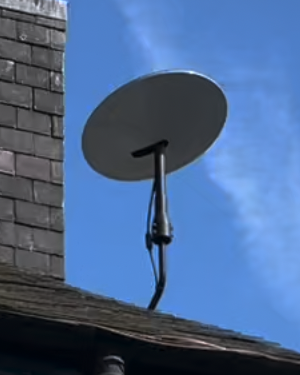
\includegraphics[width=\textwidth]{img/unstowed.png}\\\vspace{.35em}
        \centering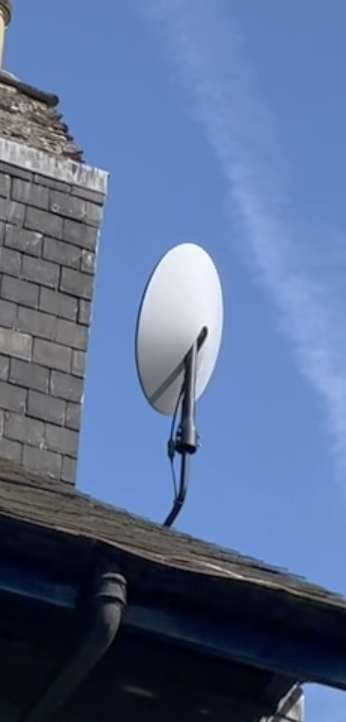
\includegraphics[width=\textwidth]{img/stowed.png}
        \caption{The dish in ``active'' (top) and ``stowed'' modes.}
    \end{subfigure}
    \begin{subfigure}{.5779\textwidth}
        \centering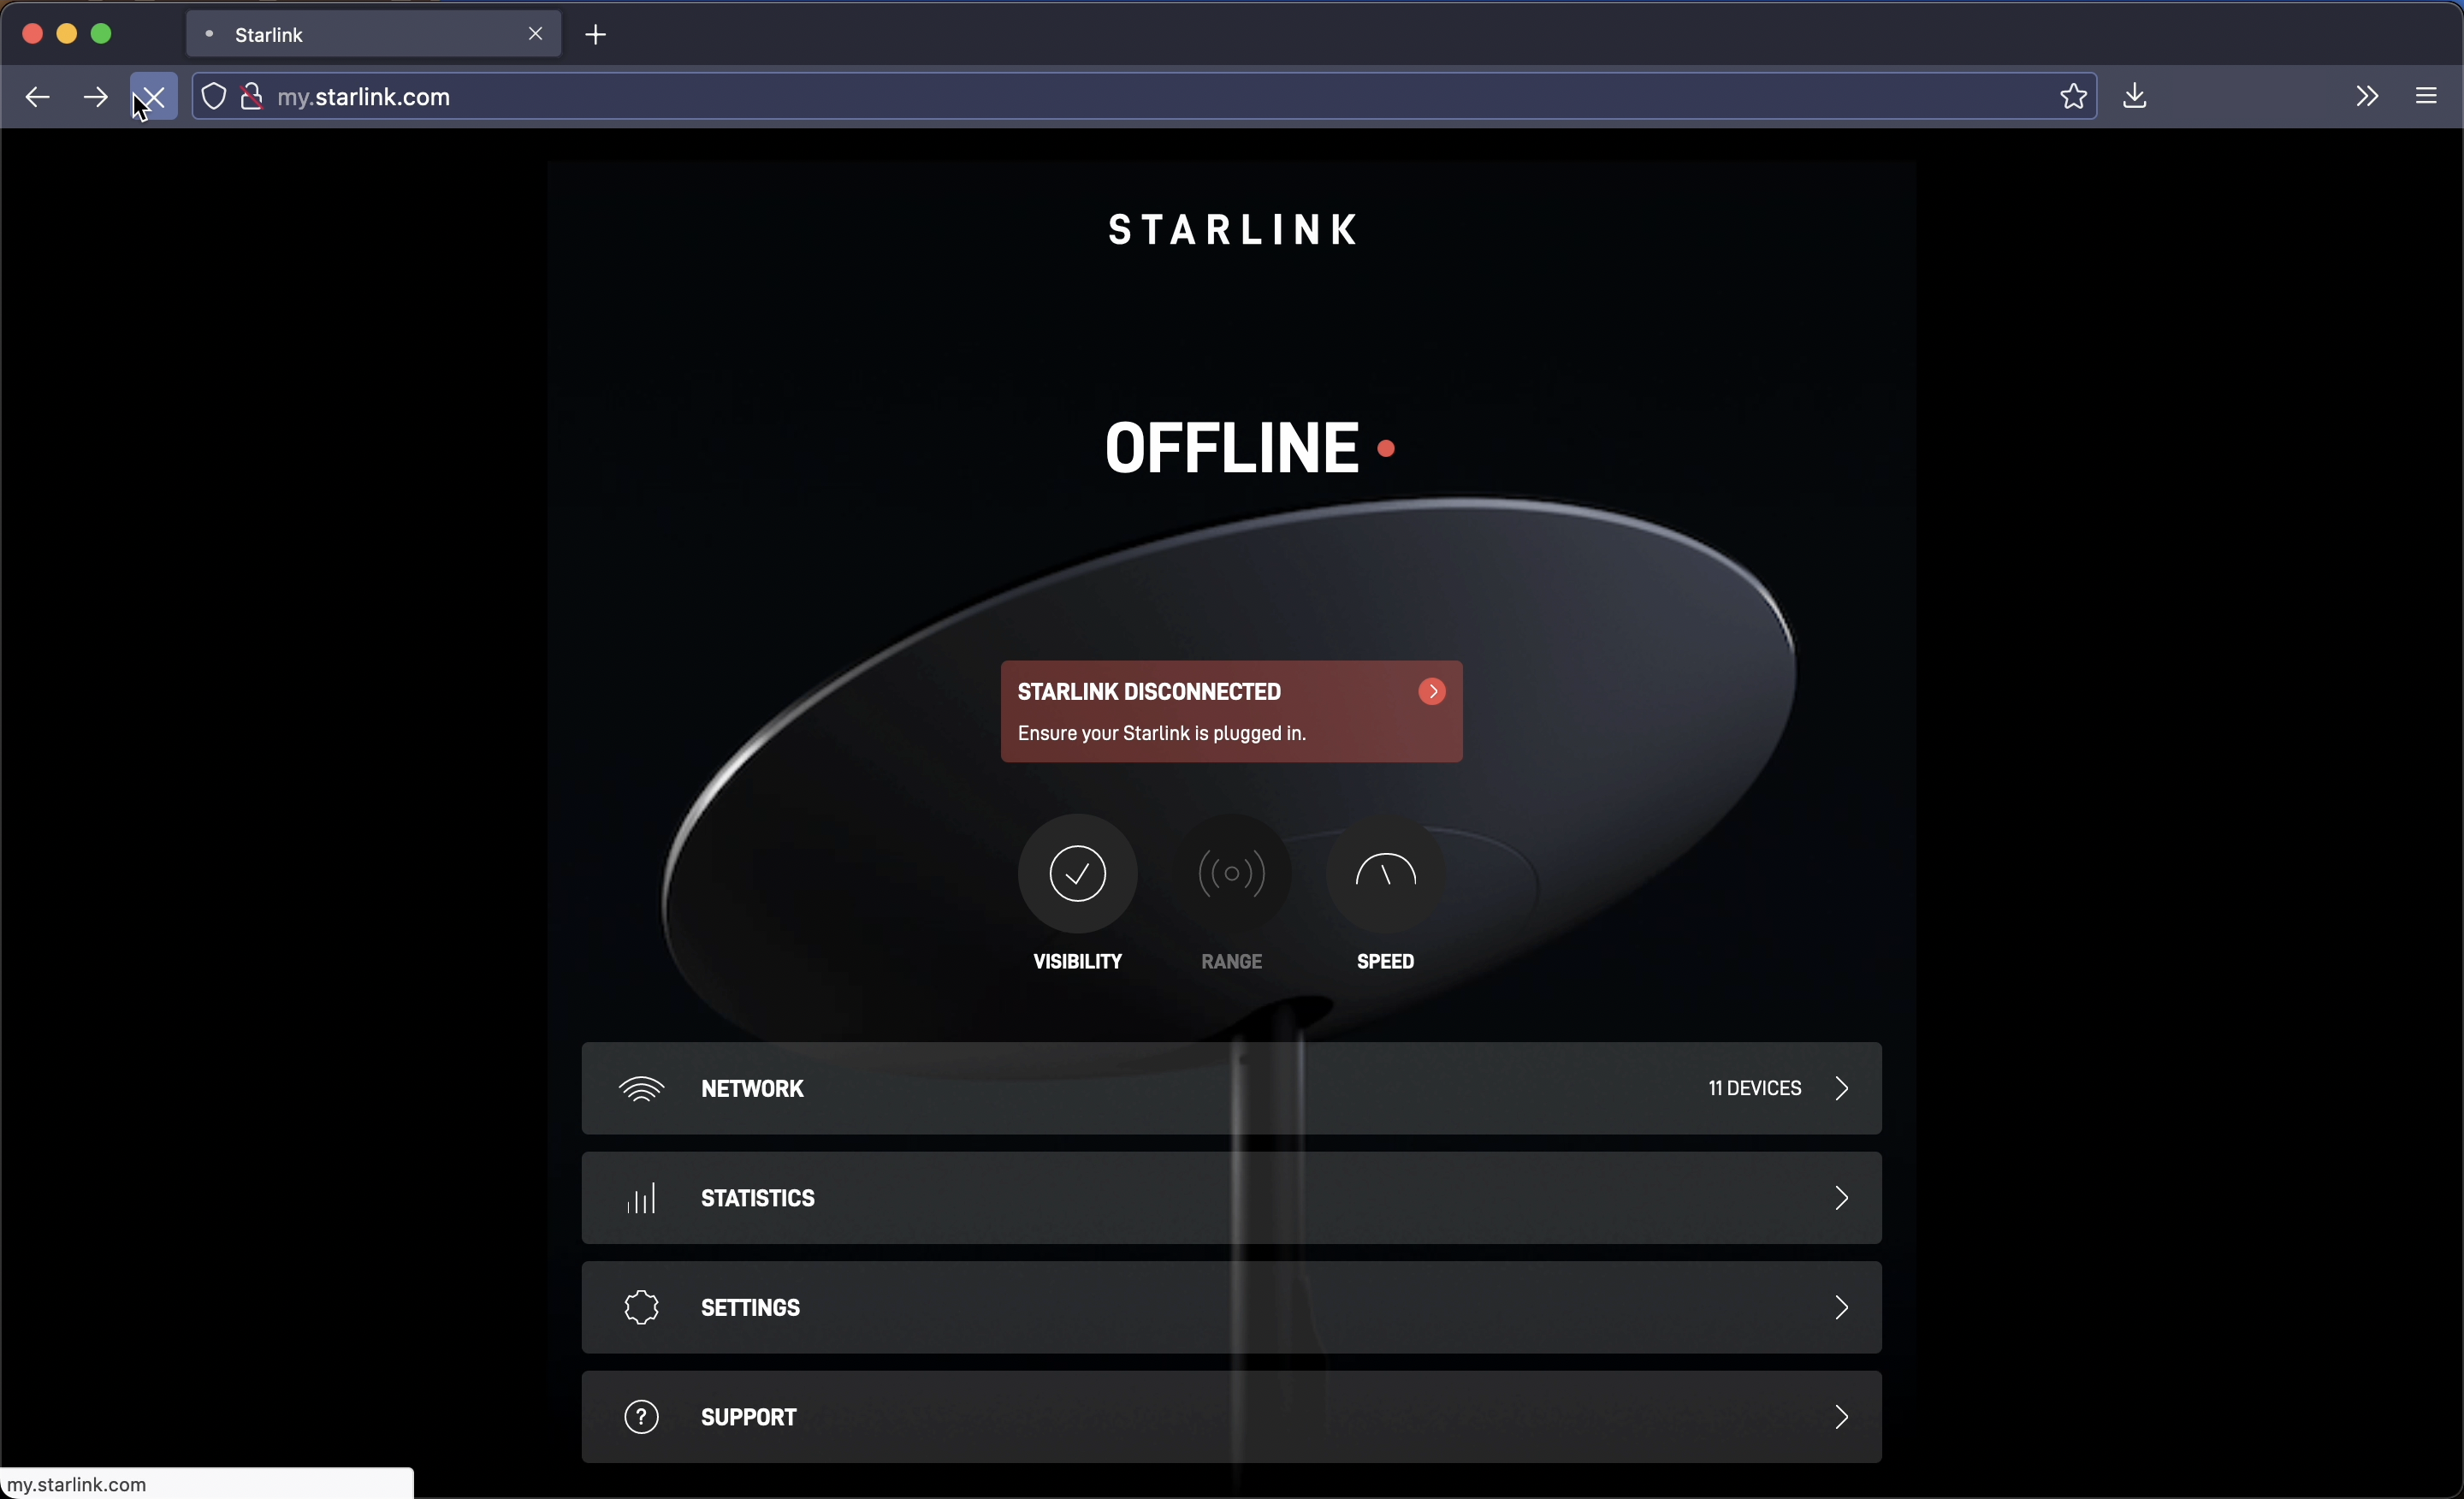
\includegraphics[width=\textwidth]{img/offline.png}\\\vspace{.35em}
        \centering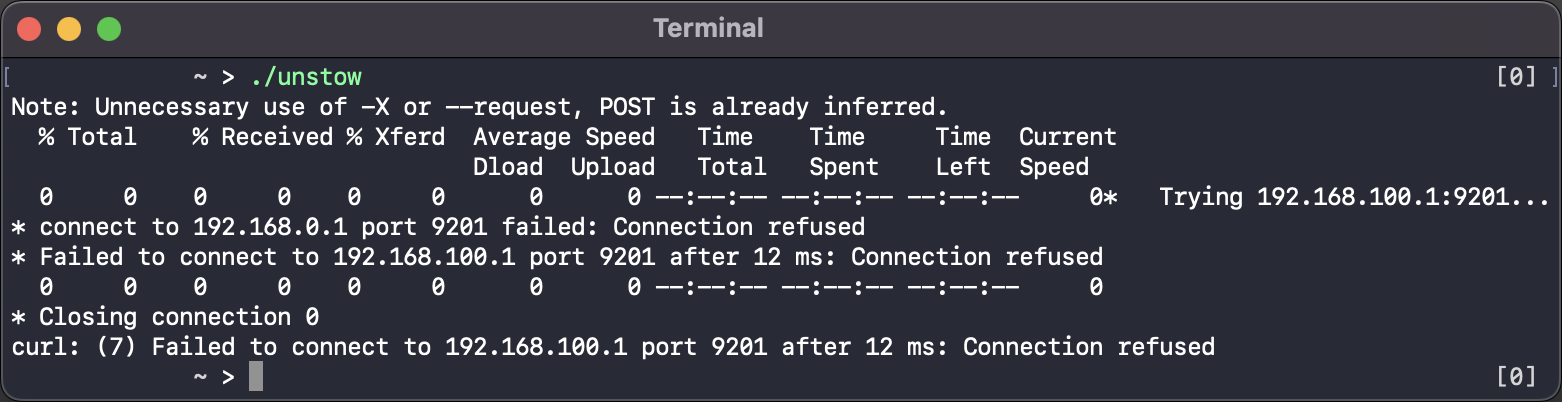
\includegraphics[width=\textwidth]{img/unstow.png}
        \caption{A screenshot of the web control panel error screen following the attack, and the result of sending commands to an inoperative dish.}
    \end{subfigure}
\caption{The outcome of a successful attack on the Starlink dish, and the resulting web control panel and response to commands.}
\label{fig:attack-outcome}
\end{figure*}

Since the modem will no longer respond to commands, the terminal is frozen in whatever state it was in before the kill command was sent.
By first sending a command to stow the dish before sending the kill command, the adversary can cause denial of service -- it will not be possible to restore internet access until the dish is physically power-cycled.

Appendices~\ref{app:stow} and~\ref{app:kill} contain shell scripts to send the stow command and the malformed kill command to a user terminal on the local network.
The outcome of this attack can be seen in Figure~\ref{fig:attack-outcome}.
